\documentclass[12pt,titlepage]{article}

\usepackage{etex}
\usepackage[english]{babel}
\usepackage[utf8]{inputenc}
\usepackage[T1]{fontenc}
\usepackage{color}
\usepackage[a4paper,lmargin={4cm},rmargin={3cm},tmargin={3cm},bmargin={3.5cm}]{geometry}
\usepackage[onehalfspacing]{setspace}
\usepackage{amssymb}
\usepackage{amsthm}
\usepackage[pdftex]{graphicx}
\usepackage{lmodern}
\usepackage{amsmath}
\usepackage{amsfonts}
\usepackage{multirow}
\usepackage{rotating}
\usepackage{mathrsfs}
\usepackage{graphicx}
\usepackage{tikz}
\usepackage{makecell}
\usepackage{vcell}
\usepackage{arydshln}
\usepackage{textcomp}
\usepackage{diagbox}
\usepackage{caption}
\usepackage{algpseudocode}
\usepackage{algorithm}
\DeclareCaptionType{equ}[][]
\usepackage[style=numeric]{biblatex}
\addbibresource{literaturechurn.bib}
\usetikzlibrary{trees}
\graphicspath{{./images/}}
\DeclareMathOperator*{\argmin}{arg\,min}


\begin{document}

\thispagestyle{empty}

\begin{titlepage}\centering
    \begin{center}
        \vspace*{\fill}
        \huge \textbf{\textsf{Customer Churn Prediction using Quotation Data}}\\
        \vspace{2cm}
        \LARGE\textbf{\textsc{Master Thesis}}\\
        \vspace{1cm}
        \normalsize
        Submitted on: \today \\
        \vspace{2.5cm}
        \large \textbf{at the University of Cologne}
        \vspace{3cm}
    \end{center}
    \normalsize{
        \begin{tabular}{ll}
            Name: & {Abdurahman Maarouf} \\
            Adress: & {Schulstrasse 31} \\
            Postcode, Area: & {53332, Bornheim} \\
            Country: & {Germany} \\
            Matriculation number: & {736481} \\
            Supervisor: & {Prof. Dr. Dominik Wied} \\
        \end{tabular}\\
    }
    \vspace*{\fill}

\end{titlepage}

\thispagestyle{empty}

\tableofcontents

\newpage

\pagenumbering{arabic}

\setcounter{page}{1}

\section{Introduction} \par

Predicting churners in order to retain customers has become one of the most important issues for companies in the field of CRM. In the ideal case, companies want to detect potential churners before they leave by estimating probabilities for a churn in the next period of time. To tackle this issue, more and more advanced Machine-Learning-Algorithms
are used guaranteeing solid accuracy in their out-of-sample predictions. \\
Fortunately for most of the companies, churn rates from one period to another are very small. However in classification
models predicting a rare event can become challenging. In this so called "Imballanced Classes" issue certain arrangements to the underlying training data or the selected objective function need be made. Without these arrangements and with highly imballanced classes, a poor algorithm will simply never predict the outcome of the minority class. In a dataset with 1000 customers containing 5 churners for example, this loss-minimizing algorithm would have an in-sample accuracy of 99.5\%. \\
In order to avoid the high amount of "False-Negative"-classifications there are many methods ranging from upsampling the
minority class or downsampling the majority class to more advanced techniques like custom loss functions. In this work we present and compare the different methods while applying them to the underlying problem. \\
We also want to emphasize the importance of using quotation data for predicting customer churn. A company can
track (potential) customer behavior on their distribution channels. Nowadays, in most cases the products or services are
offered online on websites, which makes it easy to track website visitor data. In the context of dealing with customer
churn this data can be matched to the customers already having a product or contract of this company. We show that first the number of visits of a current customer in the last period and second the average of the seen price during the visits have a high importance when predicting the probability of that customer leaving in the next period. \\
In order to evaluate the importance and relationship of not only the quotation features but also the other explanatory variables with the to-be-explained variable there is typically a trade-off during model selection. The trade-off lies between the model complexity and the model interpretability. Deep neural networks or boosted trees belong to the complex models which are famous for their comparatively high accuracy in almost all domains, espacially in computer vision and natural language processing. Understanding and interpreting the model is less important in these areas. \\ However in the course of this work and in many other areas understanding understanding how explanatory features interact with the outcome of the model becomes desirable. The most transparent models in terms of interpretability are linear or logistic models. There the magnitude and sign of the corresponding coefficients (after being testet for significance) illustrate the changes of the outcome for a change in the specific explanatory variable. These models however lack in terms of accuracy when being compared to the complex ones, because they do not allow for non-linearities and interactions in the explanatory features. Extensions, like general additive models (GAMs) \cite{gam} or GAMs allowing for pairwise interactions (GA$^{2}$Ms) \cite{ga2m} incorporate non-linearities.\\
In this work we focus on comparing the predictive accuracy and interpretability of black-box and white-box models. For the black-box model we fit gradient-boosted trees \cite{gbt} as they outperform other models in most applications with tabular data. Partial dependency plots \cite{pdp}, Shapley values \cite{shap} and LIME \cite{lime} are novel approaches designed to make these black-box models interpretable. Additionally we present the accuracy and interpretability of "Explainable Boosting Machines" (EBM) developed by Microsoft researchers Lou et al. \cite{interpretml} which are based on a GA$^{2}$Ms model and are therefore interpretable in the form of their shape functions. EBMs aim to combine the high accuracy of complex models on the one hand and the interpretability of general additive models on the other hand. \\

\section{Problem} \par

\subsection{Understanding the Problem} \par

For this work we use customer data from a big insurance company in Germany. Due to data pretection the data is anonymized which does not affect the model accuracy and interpretability in any form. We focus on the product of automobile liability insurance, which is by law a mandatory service every car owner must hold in Germany. \\
Typically car owners close a deal with an insurance company which can be terminated by the end of each year. In rare cases both sides agree on a contract with a due date during the year. If the contract does not get terminated it is automatically extended for another year. Besides the option to terminate the contract at the due date there is also an option to terminate it earlier in a few special cases. These cases mainly involve the exceptional right of termination given to a customer after a car accident or a vehicle change. To sum up, here are the two cases in which a churn can (but not must) occur before the contract due date: \\

\begin{center}
    \begin{tabular}{ll}
        Event A: & Contractor is involved in an Accident. \\
        Event N: & Contractor buys a new Car. \\
    \end{tabular}
\end{center}

The problem of modelling customer churn needs to be seperated into the probability of a costumer leaving before his contract due date and churns happening at the due date. The reason is that the optimal modelling approach and explanatory variables have differences. One example is the premium adjustment send to the customers before their due date, which has a high contribution to the decision of the customers at the due date. Meanwhile, churns before the due date are dependent on the occurence of the events $A$ and $N$. In this work we focus on predicting churns occuring before the due date. \\
This tree diagram illustrates how the probability of a churn before the due date can be decomposed using the Events $A$ (Accident), $N$ (New Car) and $C$ (Churn). \\

% Set the overall layout of the tree
\tikzstyle{level 1}=[level distance=5cm, sibling distance=3cm]
\tikzstyle{level 2}=[level distance=5cm, sibling distance=2cm]

% Define styles for bags and leafs
\tikzstyle{bag} = [text width=4em, text centered]
\tikzstyle{end} = [circle, minimum width=3pt,fill, inner sep=0pt]

% The sloped option gives rotated edge labels.
\begin{tikzpicture}[grow=right, sloped]
\node[bag] {}
    child {
        node[bag] {$None$}
            child {
                node[end, label=right:
                    {$P(None\cap \overline{Churn})$}] {}
                edge from parent
                node[above] {$P(\overline{C}\mid None)$}
            }
            child {
                node[end, label=right:
                    {$P(None\cap Churn)$}] {}
                edge from parent
                node[above] {$P(C\mid None)$}
            }
            edge from parent
            node[above] {$P(None)$}
    }
    child {
        node[bag] {$New$ $Car$}
        child {
                node[end, label=right:
                    {$P(New$ $Car\cap \overline{Churn})$}] {}
                edge from parent
                node[above] {$P(\overline{C}\mid N)$}
            }
            child {
                node[end, label=right:
                    {$P(New$ $Car\cap Churn)$}] {}
                edge from parent
                node[above] {$P(C\mid N)$}
            }
        edge from parent
            node[above] {$P(N)$}
    }
    child {
        node[bag] {$Accident$}
        child {
                node[end, label=right:
                    {$P(Accident\cap \overline{Churn})$}] {}
                edge from parent
                node[above] {$P(\overline{C}\mid A)$}
            }
            child {
                node[end, label=right:
                    {$P(Accident\cap Churn)$}] {}
                edge from parent
                node[above] {$P(C\mid A)$}
            }
        edge from parent
            node[above] {$P(A)$}
    };
\end{tikzpicture} \par

By assumption we set $P(C\mid None) = 0$ as the amount of terminated contracts during the year which are not being
caused by a new car, an accident or a due date is very small and can be omitted. Therefore we leave these cases out of our data. What we are interested in predicting is the overall probability of a churn, which can be rewritten as:

\begin{center}
    \begin{tabular}{ll}
        $P(C)$ & $=$ \hspace{3mm} $P(A\cap C) + P(N\cap C) + P(D\cap C)$ \\
        & $=$ \hspace{3mm} $P(A)P(C\mid A) + P(N)P(C\mid N) + P(D)P(C\mid D)$ \\
    \end{tabular}
\end{center} \par

One idea would be to model the three branches of $A$ and $N$ seperately. The logic behind this is that different models and sets of explanatory variables have the best fit for the probabilities of the tree branches. Not only the the branches but also the unconditional and conditional probabilities of a single branch may vary in their best modelling approach. For prediciting an accident a model of type (XY) is more suitable, whereas (YZ) would go better with modelling the probability of churn given an accident occured. In the course of this work we begin with a general modelling approach trying to predict the probability $P(C)$. At a later stage we compare the accuracy outcomes of seperately predicting the branch probabilities with the baseline approach. \\
The purpose is to build a model which can be used at any time $t$ of the year to predict the probability of a costumer leaving the company in the next period of time $(t, t+s]$ and not at his due date. It can be argued that in order to provide a model with maximized utility for production one would want to keep $s$ small. For example a company would highly benifit from a model, which can predict the churn-probability of the next week. However we see that having a small $s$ decreases the accuracy of our models, creating a trade-off situation between model accuracy and the benifits of a small $s$. With a smaller period the classes of the data become more imballanced, creating a higher challange of feeding the model enough information about churners. Furthermore, a small $s$ decreases the scope of action for a company to retain potential customers leaving. \\

\subsection{Data} \par

Most customer churn predicition models have been using only one timestamp to train a model. We want to emphasize the usage of multiple timestamps and show that it significantly improves prediction accuracy. The improvement is a result of an increased training set size and the ability of the model to especially learn more about the rare class. Furthermore, the model becomes more generalizable in time which is crucial if this model is applied in
production (see: \cite{multiplets}). Explain more using graphics.\\
Part of this work is the evaluation if the churn probability of customers is time invariant. Therefore we statistically test the equality of monthly mean churn rates. We see that there is a seasonality in the churn rate which underlines the
importance of including different timestamps in the training data for the model to learn the monthly differences. These different timestamps are simply appended to the data as additional rows creating a panel dataset. The month of these timestamps are therefore added as an explanatory feature. \\
To build the models we use historical data of the insurance company. More specifically we pick $T$ timestamps with
$t = 1,...,T$ in the past and collect all the active contracts to these timestamps. One row corresponds to one active contract at $t$. So if one hypothetical contract is active in all $T$ periods it appears as $T$ seperate rows in our data. To each row we merge the status of that contract in $t+s$, which represents the target variable. \\

\textit{Quotation Data} \par
This work stands out in its novel approach of using quotation data for churn predictions. We are not aware of similar research in the literature utilizing that data. In that sense we want to highlight its predictive power. We recommend companies and research institutions to set up systems and/or databases to collect such data. In the following we clarify what our understanding of quotation data is. Furthermore we illustrate which types of features can be generated and are used in our modelling approach.\\
Through every distribution channel a company offers its product, (potential) customers leave behind a lot of useful data. These distribution channels can either be online websites or also offline agencies. In our insurance case (potential) customers must give specific information about themselves and their car they want to insure such that a price can be calculated. Everytime a price is calculated all the information corresponding to that calculation is saved as a new row on a database. From now on we will define a price calculation as a request.\\
Main applications of quotation data involve price and new-business optimization, demand forecasting and conversion modelling. Another application however is to use this data in order to analyze the behavior of customers which already have an active contract. The main advantage of the (potential) customers having to give their and the cars information is that this information can be used to match an active customer with his/her requests. One can therefore assume that an active customer with high request activity is most likely looking for a new insurance contract. This would directly influence the churn probability. \\
The features we generate with the quotation data can be summarized into five groups: \\
\textit{(1) n\_requests$_{t - m, t}$:} To each active contract we join the number of requests generated by the corresponding customer in the $m$ months before the selected timestamp $t$. We allow for multiple values for $m$, more specifically $m \in \{ 1, 2, 3, 6, 12\}$, resulting in 5 different generated features. \\
\textit{(2) diff\_n\_requests$_{t - m, t}$:} We also calculate the average monthly number of requests in the last $m$ months subtracted by the average monthly number of requests in the last 12 months. The idea behind this group of features is that it reflects if there is a difference in request behavior of the last $m$ months to the normal behavior. So \textit{diff\_n\_requests$_{t - m, t}$} can be seen as a normalized version (using customer specific averages) of \textit{n\_requests$_{t - m, t}$}. \\
\textit{(3) avg\_calc\_price$_{t - m, t}$:} Another group of features is the average shown price of the requests. Again, we produce 5 features in this group, as $m \in \{ 1, 2, 3, 6, 12\}$. \\
\textit{(4) diff\_calc\_price$_{t - m, t}$:} Here we use \textit{avg\_calc\_price$_{t - m, t}$} and subtract it with the price the customer is paying according to his/her active contract. \\
\textit{(5) diff\_hsntsn\_requests$_{t - m, t}$:} As customers have to state vehicle specific information during their price request, this information can be compared to the vehicle which is insured in the active contract. Thereby we concentrate on the "HSN" (manufracturer key number) and "TSN" (type key number). The combination of both the "HSN" and "TSN" is a unique identifier for the type of the car. Thus, for this group of features we create a similarity score between 0 and 1. 0 reflects the case where none of the entered vehicles in the requests equals the "HSN"-"TSN"-combination in the contract and 1 is assigned to full similarity between requested car(s) and insured car. The resulting features can be an indicator for the occurence of event $N$, i.e. the customer thinking about changing his/her car. \\
Note that for each group we generate multiple features with different values for $m$. Our purpose is to find the optimal request window $m^{\star}$ for each group using a special dimension reduction technique called MRMR. This technique will be presented later and is designed to optimally filter the features when expecting correlation among them. This is highly reasonable for our quotation features.\\

- (Graphical Illustration) \\
- (Description of the ETL Process) \\
- (Description of the most important features) \\


\subsection{Literature Review} \par

There is a wide range of literature covering supervised classification techniques and their usage for customer churn predicition. Verbeke et al. \cite{verbekechurn} studies the literature on empirical churn modelling in static settings using cross-sections of data. It provides an extensive benchmark of classification methods and machine learning models applied to different data sets. \\
Other works have a different approach in modelling customer churn. Van den Poel et al. \cite{vandenpoel} for example models the time to churn using survival analysis techniques. This allows flexible estimations for the conditional probability of customer $i$ churning in the next $s$ periods of time, where the probability can be calculated for different values of $s$ by the model structure itself. Given the fact that with survival analysis, conditioning on multiple time dependent variables is not possible or not well studied yet, we will focus on modelling churn probabilities in the static setting. \\
The popularity of (deep) neural networks has risen enormously in the last two decades. Its promising accuracy in computer vision, natural language processing and sequential data in general are the reasons for its broad coverage in research. It has also found its way to modelling customer churn, as in \cite{martins}, \cite{tan2018}, \cite{wangperawong}, \cite{zaratiegui}, \cite{zhou} and \cite{mena}. All cited papers rely on the fact that customer data can be used as sequential data with time varying features. Therefore model architectures like convolutional neural networks (CNN) and long short-term memory networks (LSTM) come into play. We however focus on classification techniques which do not assume dependencies in the data points, given the data that we have available. \\
The different data preparation, preprocessing and feature engineering approaches for churn modelling are also extensively studied. \cite{coussement} for example studies the data preparation approach for modelling churn probabilities in the telecommunication industry. They suggest that an appropriate selection and engineering of features is essential to guarantee robust results and high accuracy. We apply their suggestion to some of our features, which however differ due to the different setting. \\
Regarding preprocessing, Gattermann-Itschert et al. \cite{multiplets} underline the importance of multi-slicing. This technique essantially uses multiple time-slices $T$ in the past to train the underlying models. They find out that this technique results in higher accuracy and robustness, which also holds true for our application. \\
As already stated, class imbalance naturally occurs in most churn prediction applications due to the fact that churners are less frequent than non-churners. This problematic increases in a contract-setting, where there are only a few events which allow for an earlier termination than the due date. Weiss et al. \cite{mining_rarity} provides an overview on multiple techniques to handle class-imbalance. It espacially highlights the effectiveness of sampling and cost-sensitve learning which prove to be the best techniques in our application as well. \\
Zhu et al. \cite{zhu} offers a useful guideline of sampling methods in the context of churn prediction. It compares different sampling techniques in their effectiveness and multiple evaluation metrics. Burez et al. \cite{burez} extensively underlines the importance of using appropriate evaluation metrics in a churn prediciton context. This not only increases the success of customer churn prediction models in real-life settings. It also provides trustworthy metrics in order to make models more comparable. \\
It is important to note that in the applications predictive analytics, two different evaluating approaches exist. Out-of-sample evaluation uses unseen samples from the same period(s) the model was trained on. Out-of-period evaluation tests the model on samples from a more recent period, which was not used for training. While out-of-sample evaluation is more dominant in the literature, Zahavi et al. \cite{zahavi} and Neslin et al. \cite{neslin} emphasize the importance of evaluating the performance of the model on periods beyond the ones it is trained on. \\
Out-of-period evaluation is espacially important when there are time varying factors which influence the churn rate. Examples of such factors are demand, supply, competition, inflation and pricing. Espacially in our use case with automobile liability insurance, products of competitors are close substitutes. So any change in the stated factors has high effects on customer behavior. This undermines the relevance of using multiple time slices for training and out-of-period evaluation. \\


\section{Methods} \par

In this section we present our methods of modelling churn probabilities. To fully capture the concepts we use in this work, we start with the preprocessing procedure. Then we explain used and compared methods to handle imbalanced classes. The next subsection introduces the theoretical background on the fitted machine learning models. The questions on how to evaluate these models with the appropriate metrics and how to make them interpretable are answered in the last two subsections. The modelling flow is visualized by (Figure X). \\
Put the graphical overview (from Feuerriegels slides) of the modelling pipeline (use MS Visio) here. \\

\subsection{Preprocessing} \par

As in most machine learning applications preprocessing the data is the most time consuming part in this work. To have a clean and suited training dataset for modelling and a dataset for production is essential to guarantee accurate, robust predictions and interpretations. Therefore we will present the main issues in the raw data that are solved during preprocessing. \\
The raw data comes from three main sources. The first source is a valid-time-state-table (VTST) containing all historic and present customer contracts information of the product automobile liability insurance. It contains valid-from and valid-to columns which makes it easy to extract information on the status, the car and the insurance holder at any point in time $t$. The second source table is also a VTST but contains historized accident data reported by an insurance holder. Finally, the quotation table is the third source, where simply the amount of rows equals the total number of requests generated across all distribution channels. \\
All preprocessing is done with the database language SQL for performance reasons. SQL has many advantages which makes it popular and highly demanded. It is a reliable and efficient language used for communicating with the database. Thereby it is able to process queries for data manipulation, insertions, deletions and joins fastly. \\
In order to automate the preprocessing, scripts and functions are written with python which order the sql queries in tasks and which execute them on the database. More specifically, the package "prefect" (cite) is used to create the python pipeline. It is a workflow management system primarely used for such data engineering tasks. We select prefect as it enables the option to execute the pipeline through a simple command in the console or in predefined time intervals. It is easy to monitor the process of the pipeline and it also creates an efficient overview of if there are bugs/errors in either the SQL-queries or the python scripts. \\
The preprocessing can be split up into 4 main steps and are summarized in the following: \\

\subsubsection*{(i) Creating the historized view of the Contracts}
As already mentioned, the source table containing all contract information is a VTST. So any desired point in time $t$ in the past can be selected to collect all active contracts to that time. We use $T=12$ points in time in the past, following \cite{multiplets} findings, to ensure a larger dataset and higher generalizability and robustness over time. So in the first step we generate 12 different tables, which are essantially views on the source table for the given points in time.\\
For each generated view-table (for each point in time $t$) and for each active contract we look for the status of that contract in $t+s$. This is done by joining the same table filtered for timestamp $t+s$ on the unique identifier column "contract\_number". To ensure we only collect during-contract-churns, we check if the termination date of that contract is unequal to the agreed upon termination date. The case where both dates are equal is excluded in our modelling question and therefore not seen as a churn. \\
The 12 points in time are selected carefully, in a sense that there is no overlapping between any time window $(t, t+s]$. So following property must hold for any pair of time sets: $(p, p+s] \cap (q, q+s] = \emptyset$ for all $p \neq q$ and $p,q=1,...,12$. \\
The final step for generating a historized view of the contracts is to create a union on all 12 subview, creating a panel-dataset. The number of resulting rows after this operation equals the number of rows after all next steps. So we have already generated the framework of the preprocessed table. The only thing which is left is to generate more variables, espacially accident and quotation variables. \\

\subsubsection*{(ii) Join accident data}
In many modelling problems in the insurance context it turns out that the driving behavior of the customer plays a big role in predicting the desired outcome. Espacially in risk modelling, knowing how many times a customer was involved in an accident or how costly these accidents were, ensures accurate predicitions. \\
Being involved in an accident is one of the events which give a customer the exceptional right of terminating the contract. Therefore we will also include historized accident data in the modelling approach. The VTST containing the historized accidents are recorded for each "contract\_number", which makes it easy to join the data to the table generated in (i). \\
We engineer two new features based on the accident data. One is a simple count of accident the contract holder was involved in since the start of the contract ("sum\_accidents"). The second one is the sum over the incurred costs corresponding to the accidents ("sum\_accidents\_costs"). This quantifies the accidents and makes them comparable. \\


\subsubsection*{(iii) Bot Detection in Quotation Data}

One big issue arises with the usage of quotation data. Not all requests in online distribution channels are generated by humans. The pricing information of a company is valuable for competitors pricing strategy or other third party institutions. As a result many bots or crawlers are designed to automatically extract data from websites. The proportion of not-human requests can be very high and reaches up to 70\% in one of the distribution channels. \\
As we do not want to consider bots and crawlers and falsely join them as requests from our active customers we need to find a way to detect them. The first best strategy would be to label a proportion of requests as $BOT=True$ or $BOT=False$ and then train a model to estimate $P(BOT=TRUE \mid X)$ for the remaining requests. This however is infeasible as there is no information on the true labeling for any request. \\
The second best approach flags requests with unreasonably high number of same occurences and is used in this work. Thus, it counts the number of requests with the same combination of certain quotation features (1) over a day and (2) over the entire timeframe. These features for flagging bots/crawlers should be as unique as possible in a sense that requests coming from the same source are only counted. For both (1) and (2) individually, a certain cutoff percentile of the combinations is specified. A request is then specified as a bot if the rank of its specific combination is larger than the cutoff. \\
The cutoff percentile is defined for every distribution channel individually (as some are more prone for bots than others). How to choose the "correct" cutoff is done through eyeballing the smoothness of distributions for suitable quotation features. An example is the feature "time\_of\_day", where we have an expected distribution and can detect anomalies with our eye. \\
Figure X represents the result of the bot detection algorithm and the distribution of "time\_of\_day" over the entire time since 2018 for one specific online distribution channel. It is a screenshot of the dashboard which is used to monitor the performance of the algortihm. It was also used to finetune the cutoffs for every distribution channel and to choose the right combination of features. The spikes between 2:30 am and 4:30 am clearly represent such an anomaly and are fully captured by our bot detection algorithm. \\
\centerline{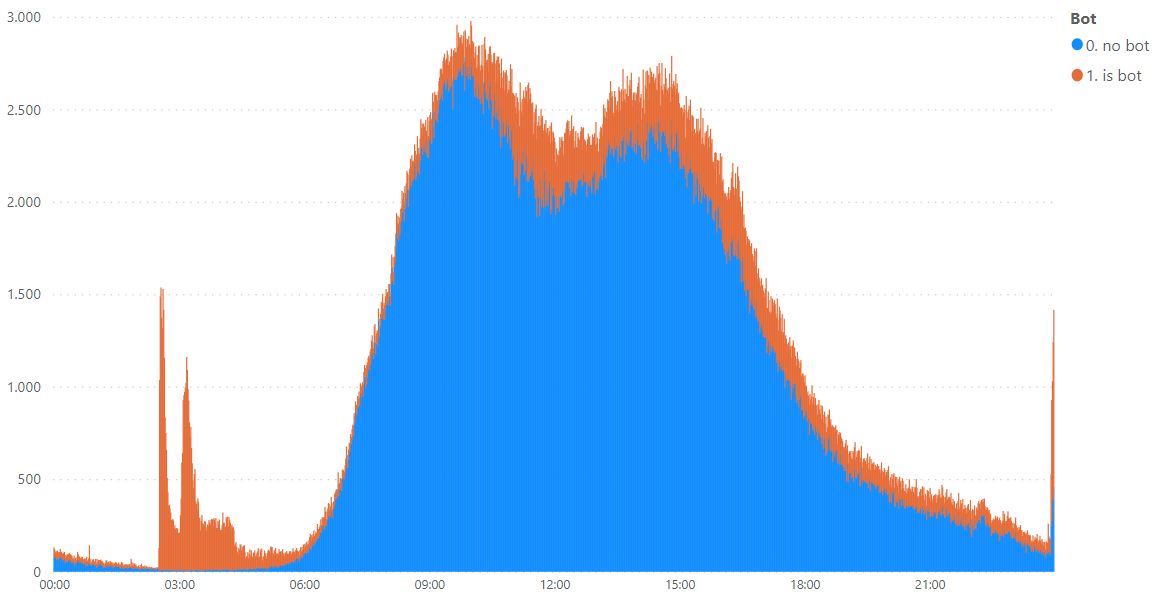
\includegraphics[height=8cm]{bots_day_time.png}}

The advantage of this algorithm is that it also captures newly arriving bots by calculating percentiles per day. Also it is able to treat the distribution channels individually. It is easily adjustable and monitorable. It however still fails to capture certain types of bots which are programmed to enter a different combination of features in each request. There however, it is nearly infeasible to detect them with any advanced method. In this work we estimate that these bots only make up a very small fraction of the requests and therefore we neglect them. \\

\subsubsection*{(iv) Matching quotation with contract data}
Another issue with the quotation data is that there is no unique identifier column which can be used to correctly join it to the table generated in (i) and (ii). Additionally, columns like $NAME$ or $BIRTHDATE$ are not always correctly specified during their price request which makes the matching even more difficult. If specified correctly in the quotation data, a combination of these variables could be used as key columns. \\
In order to adress this $M\times N$-Matching problem we need to come up with a fuzzy matching algorithm. On one side we have a table which contains contracts at different timestamps, their status 2 months later and historic accident information. At the other side we have an ungrouped and unstructured table which simply lists all requests and their corresponding request information. The end result should be of the same structure as the base table created in (i) and (ii) but simply appended with the variables mentioned in (3.1???). We can already expect, that not all contracts have quotation activity $m$ months before $t$. Also, not every request is associated with a contract holder. These two facts increase the uncertainty of matching but are necessary to check the scope and quality of matching. \\
The main idea behind our fuzzy-matching algorithm is to try to match both tables with a different set of signals iteratively. Each signal is a collection of variables which together serve as almost unique identifiers. One example for a signal is the combination of the variables: $HSN$ (manufracturer key number), $TSN$ (type key number), $PLZ$ (postal code) and $BIRTHDATE$. \\
As we join the quotation table on the contract table multiple times with different sets of signals we expect and first allow for duplicates of same contract$\times$timestamp combinations and/or requests. Therefore the next important step in this section is the deduplication. We know that first the combination of contract\_id$\times$timestamp and second request\_id should be unique in the end table. \\
The first step of deduplication is to only include requests for each contract, which occured in the corresponding request window $[t-m,t)$. As we allow for different values for $m$ we first set the filter to the maximum length of $m=12$. The different variables are generated in a later step. \\
The matching algorithm is designed in a way that it implicitly allows to formulate preferences about the matching signals. So to each signal a preference rank is associated. This is used for the second step of deduplication. To further eliminate duplicates, we only keep the most preferred match per contract\_id$\times$timestamp combination on the one hand and per request\_id on the other. \\
After the second deduplication step there might still be unwanted duplicates if for example the same requests are joined to different contracts with the same signal preference. To address this last issue we pick the request-contract pair with the smallest time difference. This of course is not always the correct pair, but ensures wrong duplicates. Additionally there is no other information to be exploited for correct matches. Unwanted duplicates occuring after deduplication steps 1 and 2 are however very rare (0.002\%) and therefore can be neglected. \\
After these steps we are left with generating the quotation features mentioned in (3.1???). The result is a table with same length as after step (i) and (ii) and with appended quotation features. \\

As for the bot detection we generate a dashboard to monitor the quality of the matching algorithm. We have developped three checks which automatically are executed everytime the preprocessing is performed. We will present them shortly in the following. \\
For all the checks we exploit the fact that every new-business contract, so a newly closed deal between customer and insurance, needs a corresponding request in the quotation data. Therefore we use the same matching algorithm, but instead of joining the quotation data on our base contract table from (i) and (ii) we join it on a new-business table, which is also given in our database. With a perfect matching algorithm we would expect a match rate of 100\%. While monitoring our algorithm a match rate of 100\% should however be regarded critcially as it might be a result of too weak signals. \\
The first check is done by eyeballing the aggregated match-rate of the new-business-contracts over time. In the below graph the x-axis represents the starting date of the new-business contracts and the y-axis the match rate to these contracts. The graph shows that the performance of the algorithm is stable and accurate as in the entire time window for over 90\% of the contracts the corresponding request is found. The drop after November 2021 should not be misinterpreted as the plot was generated in November. \\

\centerline{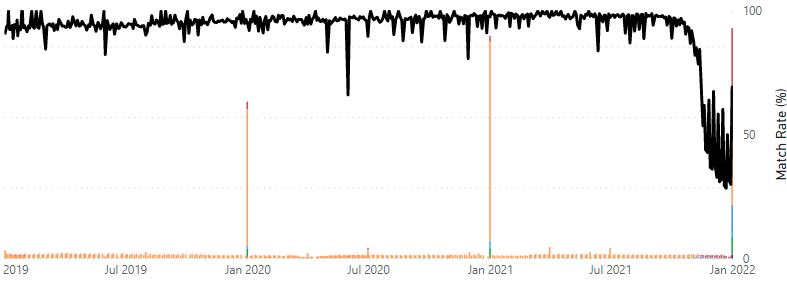
\includegraphics[height=6cm]{matching.png}}

To also ensure the correctness of the matches we monitor the quality by comparing the price determined in the new-business contract with the price of the matched request. Prices are not used in any matching signal for two reasons. One is the fact that after a converted request there may occur specific rebates or other changes to the price which lead to differences between contract price and request price. The second reason is to have an unbiased check of the matching-quality. \\
The resulting second check is a visual where the percentage deviation between contract price and request price are binned into buckets for all new-business contracts. We expect some deviation around plus and minus 20\% for given reasons. Abnormal differences over the 20\% mark indicate a bad match. \\

\centerline{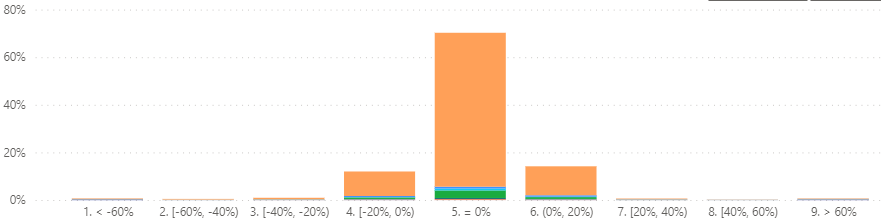
\includegraphics[height=5cm]{quality.png}}

As we can see, after optimizing the matching signals and preferences bad matches occur in only a very small proportion.Additionally we can safely say that a minimum of 70\% of the contracts are correctly matched with its request as prices are exactly equal in these cases. Adding the expected deviation of contract and request price we are left with a good quality of matching.\\
The third check also uses the new-business contracts as a test table for the performance of the algorithm. The idea behind this check is however to ensure that the current implementation is the best possible with the underlying data. \\
We therefore model the match status (boolean) of the new-business contract as target variable and all underlying quotation and contract variables as explanatory variables. The model itself is a decision tree. The defining rule to decide wether the algorithm is using the most out of the given information is the resulting feature importance score. More specifically we use the score which assigns its overall contribution to loss reduction to each feature. So for each feature we calculate the decrease in node impurity weighted by the probability of reaching that node.\\
Under full exploitation of the information at hand the decision tree should not be able to find a structure to model the match boolean. In result we should expect complete randomness in the structure of the tree and almost equal feature importance scores for all the features. If there is any feature with abnormal high feature importance it is a sign for incomplete information usage for matching. \\


\subsection{Dimension Reduction} \par

A full collection of the explanatory features in our data can be found in the appendix. As we have many features and some of them are highly correlated, preprocessing this dataset is essential. The goal is to retain only the minimal optimal subset of features. In many cases, due to multicollinearity in models with many features, dimension reduction techniques can even improve the accuracy of models. \\
In the current literature of machine learning there are many approaches for feature selection, ranging from manual selection to fully automated selection procedures. We use the "Maximum Relevance Minimum Redundancy" (MRMR) - approach designed by Ubers machine-learning researchers Zhao et al. \cite{mrmr}. The authors focus on designing an algorithm which detects the best subset of features instead of the subset of best features. The latter is often used in applications of machine learning, where a model is trained and features are selected a posteriori based on certain feature importance scores for that model. This however does not eliminate redundant features, which in reality do not improve the model performance due to being already represented in correlated other input features. \\
Using the best subset of features also helps us to identify the optimal length of the request window $m$. As we want to examine the impact of quotation data for predicting customer churn, we include multiple number-of-request features with different values for $m$ in our unfiltered selection of features $F$. These are obviously expected to be highly correlated, which additionally delivers a possibility to monitor the effectiveness of the MRMR. \\
MRMR works iteratively, so at each iteration a new best feature is identified and added to the list of selected features. Once a feature is selected it cannot ever be unselected in the next iterations. One drawback of this approach is that the number of iterations and therefore the number of selected features has to be predefined. We extend it however in a way that we iterate through the entire feature set $F$ and cache the resulting sets and scores of each iteration. So the resulting iterative process starts with an empty selected $S$ and full unselected $U$ set and ends with a full $S$ and an empty $U$. This lets us define the optimal number of iterations retroactively. \\
The algorithm MRMR got his name from the fact, that at each iteration $j$ a new feature is selected into $S$ that has the maximum relevance with respect to the target variable scaled by the redundancy with respect to the features that are already in $S$. Therefore at each iteration and for each of the remaining features of $U$ the following score is computed: \\

\begin{equation} \label{score_raw}
    score_{i}(feature_{i \in U}) = \frac{relevance(feature_{i \in U}, C)}{redundancy(feature_{i \in U}, features \in S)} \\
\end{equation}

The sets $U$ and $S$ get updated each iteration by transfering the feature with the highest score from $U$ to $S$. In their paper, Zhao et al. present multiple metrics for both relevance and redundancy. We focus on one approach which yielded the best result in their paper and slightly adapt it to our problem, as we have categorical features in our data. \\
At each iteration the relevance of the remaining features in $U$ has to be computed with a new model with only these remaining features. We use gradient boosted trees and its package "lightgbm" (LGBM) in python in each iteration to score the new relevance of each remaining feature. LGBM can handle categorical features on the one hand and has a build in method for calculating feature importance on the other hand. There, feature importance is computed as the number of times that specific feature is selected for a split. So this feature importance is assigned to the corresponding features as the relevance score. How gradient boosted trees work is explained in chapter 3.4. \\
For redundancy an average over certain standardized metrics for the relationship between the to be evaluated feature and the features already in $S$ needs to be computed. These metrics depend on the scales of measurement for the features. Zhao et al. only cover the case of continuous features and their relationship. We extend the redundancy score to categorical and dichotomous features. Thereby we need to pay attention to the fact, that the scores need to stay comparable for the different scales. Therefore the chosen metrics are all standardized to values between 0 and 1, where 0 indicates no and 1 the strongest possible relationship. The different scale-pairs and their relationship metrics can be summarized by table 1 (see \cite{correlation}): \\

\setlength{\tabcolsep}{10pt} % Default value: 6pt
\renewcommand{\arraystretch}{1.5}

\begin{table}
    \centering
    \caption{Relationship Metric based on Scale}
    \begin{tabular}{l|l|l|l}
    \diagbox{}{} & nominal & dichotomous & continuous      \\
    \hline
    nominal                & Cramers-V-Correlation &         &                 \\
    \hline
    dichotomous            & Cramers-V-Correlation & Cramers-V-Correlation &                 \\
    \hline
    continuous             & Eta-Correlation & Point-Biserial-Correlation & Bravais-Pearson-Correlation
\end{tabular}
\end{table}

Redundancy is then calculated by the mean of the relationship scores as follows: \\

\begin{equation} \label{redundancy}
    Redundancy(feature_{i \in U}, features \in S) = \frac{1}{n(S)} \sum_{s=1}^{n(S)} relationship(i, s)
\end{equation}

The slightly modified MRMR-approach we use can therefore be illustrated by this simplified pseudo-code: \\
\begin{algorithm}
\caption{MRMR-Algortihm}\label{alg:mrmr}
\begin{algorithmic}
    \State $corrmatrix \gets corr(X)$
    \State $S \gets \left[ \right]$
    \State $U \gets \left[X.columns\right]$
    \State $cachedict \gets \{\}$
    \For{j in range len(X.columns)}
        \State $relvector \gets LGBMscorer(U)$
        \State $redvector \gets mean(corrmatrix\left[U\right]\left[S\right])$
        \State $scorevector \gets relvector/redvector$
        \State $bestfeat \gets max(scorevector).name$
        \State $bestscore \gets max(scorevector)$
        \State $S.append(bestfeat)$
        \State $U.drop(bestfeat)$
        \State $cachedict.append(j,bestfeat, bestscore)$
    \EndFor
\end{algorithmic}
\end{algorithm}
- The results of MRMR for our dataset are as follows: Show using graphics of average score of each iteration. Argue with an elbow criterium? \\

\subsection{Handling Class Imbalance} \par

Studying the rarity of an event in the context of machine learning has become an important challange in the recent two decades. Rare events, such as a customer churning in the next period, are much harder to identify and learn for most of the models. HaiYing Wang et al. \cite{convergence_rareevents} study the convergence rate and distributaional properties of a Maximum-Likelihood estimator for the parameters of a logistic regression while prediciting rare events. Their finding is that the convergence rate of the MLE is equal to the inverse of the number of examples in the minority class rather then the overall size of the training data set. So the accuracy of the estimates for the parameters is limited to the available information on the minority class, even if the size of the dataset is massive. \\
Therefore some methods have been developed to decrease the problematic of imballanced classes. In this chapter we present different methods which can be applied to the training set, before feeding it to the model. Also, we present different objective loss functions which also aim in solving the problematic. To handle and evaluate the outcomes
of prediciting rare events also the appropriate models and model evaluation metrics must be chosen. This is discussed in the next two subsections however. \\

\subsubsection*{(i) Downsampling}

The first basic sampling method is named downsampling. It randomly eliminates examples from the majority class in order to artifficially decrease the imballance between the two classes. The downside of this approach is that it possibly eliminates useful examples for the model to maintain a high accuracy in predicting the majority class \cite{mining_rarity}. HaiYing Wang et al. also study the convergence rate and distributaional properties when applying downsampling. According to their findings the asymptotic distribution of the resulting parameters may be identical to the MLE's using the full data set. Under this condition there is no loss in terms of efficiency (minimum possible variance of an unbiased estimator devided by its actual variance). \\

\subsubsection*{(ii) Upsampling}

The second basic sampling method is the upsampling approach. This method simply duplicates examples from the minority class until the classes are more balanced. While duplicating examples though, the chances of overfitting to these duplicates becomes a more probable threat. Also, no new data is being generated in order to let the model learn more valuable features about the minority class \cite{mining_rarity}. Additionally, the computational performance of this approach can get rather poor, espacially with large datasets and highly imballanced classes. While evaluating the asymptotics of the MLE's with upsampling, HaiYing Wang et al find out that it also decreases the efficiency. A probable higher asymptotic variance of the estimators is the reason for that. \\

\subsubsection*{(iii) SMOTE}

The more advanced SMOTE-approach (Synthetic Minority Oversampling Technique) \cite{smote} also creates more artifficial examples of the minority class. Instead of simply duplicating some rows SMOTE creates new nearest neighbors in terms of feature values for the minority class examples. While constructing the feature values of the new example $(N + 1)$ (where N is the size of the unsampled dataset) as a new nearest neighbor for example $i$ of the
minority class one has to differentiate between continuous and nominal features. The k-nearest neighbors for the minority class are typically constructed with the Euclidean Distance for continuous features and the Value Distance Metric for nominal features (TODO: maybe include other distance measures here? Mahalanobis Distance to calculate out correlation?).
\vspace{3mm}

\textbf{A. Continuous features:} \\
1) Construct difference between corresponding feature value of example $i$ and one of its k nearest neighbors. \\
2) Multiply this difference with a random value drawn from a uniform distribution between 0 and 1. \\
3) Construct the feature value of the new example by adding the multiplied difference to the feature value of example $i$.
\vspace{3mm}

\textbf{B. Nominal features:} \\
1) Choose the feature value which is the majority vote between the feature value $i$ and its k nearest neighbors. \\
2) Assign this value to the corresponding feature of the new example. \vspace{3mm}

With this approach it is ensured that the model learns more about the neighborhood regions of the minority class. It decreases the probability, that the model overfits to the duplicates created in upsampling. \\

\subsubsection*{(iv) Cost-Sensitive Classifiers} \label{Cost-Sensitive Classifiers}
One drawback of the presented sampling methods is that the sample distribution is being changed. A different starting point is to change the objective loss function which is minimized during the model fitting. Thereby the sample size and the distribution stay the same. In the modified cost function we want to penalize false-negative
classifications with a higher weight. Reason behind this is to ensure that the event of interest, represented by the minority class, is predicted correctly \cite{cost_sensitive}. \\
The challange of this approach is to find the appropriate penalty parameters. It is hard to measure the cost of misclassifying an insurance-customer regarding churn-probabilities. The fact that these costs can come from multiple sources which are not easily definable is one part of the reasoning. Therefore we focus on two types of modified loss functions.\\
One conventional method is to assign simple parameter weights $w0$ and $w1$ to the loss function. By default one might use the inverse of the class frequency as the associated weights. These parameters however can also be optimized during grid search. We call this method the "Simple Weighted Loss Function". The derivation is part of the next subchapter.\\
The second approach is called "Focal Loss Function" and was originally designed by FAIR (Facebook Artifficial Intelligence Research) for an object detection purpose \cite{focal}. As it also aims to penalize false-negative classifications it is widely used for predicting rare events. Again, the exact structure is shown in the next subchapter and the parameters can be tuned with grid search.\\


\subsection{Machine Learning Models} \par

In this section we will present and explain mathematical and statistical theoretics behind the machine learning approaches used to model churn in this work. As already stated, the two modelling approaches in this work are gradient boosted trees (GBT) and explainable boosting machines (EBM). GBT are selected due to its known predictive accuracy on tabular data. We compare it to EBM, which essantially aims to provide an explainable model structure. \\
In order to provide the mathematical and statistical intuition behind GBT and EBM, less complex models have to be explained first as they build upon them. That is why we start with logistic regression and classification trees and work our way up to the more complex models. \\

\subsubsection*{(i) Logisitic Regression}
The logistic regression is used as a benchmark model for all classification problems. It has high advantages in terms of computational complexity and interpretability, but fails in capturing complex relationships and interactions. As it has the lowest accuracy of all classifiers it is mostly used as a baseline model in order to evaluate the advantages of additional complexity in the models, as in GBT and EBM. We however use a different baseline in our modelling approach and therefore only introduce it as the logic is needed for the more complex models.\\
Logisitic regression applies a sigmoid function to the linear regression model in order to get output values (probabilities) between $0$ and $1$ as in a Bernoulli distribution. We use the following conventional notation throughout this work: \\

\begin{equation} \label{bern_dist}
    \widehat{C_{t+s}} = P(C_{t+s}=1\mid X_{t}) = f\big(g(X_{t})\big) = \frac{e^{g(X_{t})}}{1 + e^{g(X_{t})}} \\
\end{equation}

Note that from now on we use a vectorized notation. So $\hat{C}$ represents a vector of probabilities, where the i'th element ($i = 1,...,N$) corresponds to the probability of a churn in time $t+s$ of the same at $t$ active contract. This probability vector is constructed by a model conditional on a feature matrix $X$ at time $t$. Again, each row of $X$ represents a different contract and column j is the feature j ($j = 1,...,M$) of that contract. \\
Therefore $f(\cdot)$ is the sigmoid function used on function $g(\cdot)$, where in logistic regression $g(\cdot)$ is a linear model. For GBM and EBM this function is allowed to be more complex. \\

\begin{equation} \label{lin_model}
    g(X_{t}) = \beta X_{t} + \epsilon_{t} \\
\end{equation}

Maximum Likelihood is then used to estimate the vector of parameters $\beta$ of the model. It maximizes the joint probability that the status of the training data contracts are drawn from the Bernoulli distribution stated in (\ref{bern_dist}). For the final model in production, when estimating probabilities for a churn in the next period, $t$ is of course equal across all contracts in $X$. But as already stated, for training the model we use multiple timestamps of the historized data. Therefore the index $t$ is left out for the input matrix $X$ and output vector $C$ while estimating model parameters, avoiding a misleading notation. Still, the status of contract $i$ is determined after $s$ units of time for all contracts. The likelihood function to be maximized is described as follows: \\

\begin{equation} \label{logistic_MLE}
    \mathcal{L}(C; X, \beta) = \prod_{i=1}^{N}P\big(C^{(i)}=1\mid X^{(i)}\big)^{I(C^{(i)}=1)}\Big(1 - P\big(C^{(i)}=1\mid X^{(i)}\big)^{1 - I(C^{(i)}=1)}\Big) \\
\end{equation}

To describe this term as a loss function it is characterized by the negative logarithm of (\ref{logistic_MLE}), which can be minimized with respect to $\beta$ using Gradient Descent, Newton Raphson (Zitieren!) or other optimization methods.

\begin{equation} \label{logistic_log_MLE}
    \begin{aligned}
        l(C; X, \beta) & = -\sum_{i=1}^{N}C^{(i)}log\big(P(C^{(i)}=1\mid X^{(i)})\big) + (1 - C^{(i)})log\big(1 - P(C^{(i)}=1\mid  X^{(i)})\big) \\
        & = -\sum_{i=1}^{N}C^{(i)}log(\widehat{C^{(i)}}) + (1 - C^{(i)})log(1 - \widehat{C^{(i)}}) \\
    \end{aligned}
\end{equation}

In our case we have a lot of features in the raw matrix $X$. Consequently it makes sense to add a penalty term to the loss function to avoid overfitting to the training data. While minimizing this loss function during training, this additional penalty term either shrinks some parameters of $\beta$ towards zero (L2 regularization), or sets some to exact 0 (L1 regularization). However, we can also reduce the dimension of features prior to fitting the model, as already explained with the MRMR-approach. \\
Additionally, as already mentioned in (\ref{Cost-Sensitive Classifiers}), one technique to handle imbalanced classes is to use cost-sensitive classifiers. We can implement this by setting additional penalty weights to our loss function. The resulting objective "Simple Weighted Loss Function" is described as:\\

\begin{equ}[!ht]
\caption{Simple Weighted Loss Function}
\begin{equation} \label{loss_fct_wl}
    L(C, \widehat{C}) = -\sum_{i=1}^{N}w_{1}C^{(i)}log(\widehat{C^{(i)}}) + w_{0}(1 - C^{(i)})log(1 - \widehat{C^{(i)}}) + \lambda h(\beta)
\end{equation}
\end{equ}

Here, the penalty term $h(\cdot)$ can either be an L1 or L2 regularization on $\beta$. The additional parameters of $\lambda$, $w_{0}$ and $w_{1}$ are hyperparameters which can be tuned during grid search. Following (whose?) approach, $w_{1}$ and $w_{0}$ can also be set by default to the inverse of their corresponding class frequencies in the training data. \\
The objective "Focal Loss Function" is set up like this: \\

\begin{equ}[!ht]
\caption{Focal Loss Function}
\begin{equation} \label{loss_fct_fl}
    L(C, \widehat{C}) = -\sum_{i=1}^{N}\alpha(1 - \widehat{C^{(i)}})^{\gamma}C^{(i)}log(\widehat{C^{(i)}}) + (1 - \alpha)\widehat{C^{(i)}}^{\gamma}(1 - C^{(i)})log(1 - \widehat{C^{(i)}}) + \lambda h(\beta)
\end{equation}
\end{equ}

Again, $\lambda$, $\alpha$ and $\gamma$ are hyperparamaters, which can be optimized during grid search. We use and compare both \ref{loss_fct_wl} and \ref{loss_fct_fl} for our classifiers to get the best out-of-sample performance. \\
After having found the optimal set of parameters it is time to define the classification cutoff $\tau$ for predicting a churn. The logistic regression model outputs a probability which is between 0 and 1. The rule of thumb is to set $\tau = 0.5$, such that probabilities larger than $0.5$ are predicted as churns and the rest as non-churns. \\
- Interpretability of Logistic Regression runterschreiben \\

\subsubsection*{(ii) Tree-based Classifier}

\textit{Single Classification Tree}

Classification trees have a different approach on builing a prediction model for $\widehat{C_{t+s}} = P(C_{t+s}=1\mid X_{t})$. Unlike linear or logistic regression, they allow for non-linearities and interactions. Classification trees search for the optimal sequential binary sample splits in order to minimize an objective loss function. So at each node of the tree the optimal feature $j$ and its optimal split point $r$ need to be found. The search at each node can be summarized as follows:

\begin{equation} \label{dec_tree}
    \begin{aligned}
        S_{1}(j, r) = \{X\mid X^{j}\geq r\} , S_{2}(j, r) = \{X\mid X^{j}< r\} \\
        \{j, r\} \in \argmin_{j, r} \sum_{i:X^{(i)}\in S_{1}(j, r)}l(C^{(i)}; X^{(i)}, \widehat{p^{k}}) + \sum_{i:X^{(i)}\in S_{2}(j, r)}l(C^{(i)}; X^{(i)}, \widehat{p^{k}})
    \end{aligned}
\end{equation}

The loss function for region $S_{k}$ is calculated using the resulting region prediction $\hat{p^{k}}$ (applied to all obeservations which are assigned to this region after the splits $i:X^{(i)}\in S_{k}$), which are simply the shares of churns in $S_{k}$. The typical loss functions are based on evaluating the purity of the resulting regions. In the ideal case, one would like to find the splits in $X$ which always correctly assign contracts of the two classes into two different regions. In this case, $\hat{p^{k}}$ would always be either 1 or 0. In order to approach this case one either uses the Gini-index or the Cross-entropy for region $S_{k}$: \\

\begin{center}
    \begin{tabular}{ll}
        Gini-index: & $2\widehat{p^{k}}(1-\widehat{p^{k}})$ \\
        Cross-entropy: & $-\widehat{p^{k}}log(\widehat{p^{k}}) - (1-\widehat{p^{k}})log(1-\widehat{p^{k}})$ \\
    \end{tabular}
\end{center}

The splits at each node are performed until certain criteria for the loss functions or other hyperparamaters are met. Hyperparameters of a single tree are summarized in table 2. To get the prediction $\hat{C^{(i)}}$, one assigns $\hat{p^{k}}$ as the region prediction of the corresponding end node of observation $i$ to that value. \\

\textit{Boosted Trees for Classification}

In most applications the predictions of a single classification tree have high variance due to overfitting to the training data. The accuracy in the prediction on unseen data will therefore be rather poor compared to the accuracy during training. Random forests \cite{randomforest} are designed to reduce the variance of the predictions, by averaging over predictions of multiple independent trees. This phenomenon is called "Wisdom of the Crowds" and is underlined by the fact that the average of multiple estimators for the same parameter will have the same bias but a smaller variance (how much depends on N and the correlation (which is 0 if we assume that the base learners are independent) of the estimators) than a single estimator. \\
The current literature (cite!!!) however agrees on the fact that Boosted Tree Algorithms outperform Random Forests, and therefore also a single tree. Therefore we focus on the core methodology and hyperparameters of boosted trees in the following. \\
The idea of boosted trees for classification is to have a sequence of dependent base learners (trees), which improve in terms of accuracy where it is most needed. Thereby, the base learners $\hat{g}_{b}(X)$ ($b=1,..,B$) are constructed in a shallow shape, avoiding an overfitted single learner. Additionally the $\hat{g}_{b}(X)$ are now regression trees, which output values in $(-\infty, \infty)$. So for the optimal split at the nodes of each tree the squared error reduction of the log-odds? (besser erklären, bzw statt classification trees einfach regression trees einführen?) are now being compared. To get an interpretable result we again have to apply the sigmoid function $f(\cdot)$ to get a probability in $[0, 1]$. The resulting loss of each tree is then fitted by the preceeding trees. So the procedure can be summarized by this pseudo code: \\

\begin{algorithm}
\caption{Boosted-Trees-Algortihm}\label{alg:boostedtrees}
\begin{algorithmic}
    \State $\hat{G}(X) \gets 0$
    \State $L \gets \sum_{i=1}^{N} l(C^{(i)}, f(\hat{G}(X^{(i)})))$
    \For{b in range(1, B)}
        \State Fit tree $\hat{g}_{b}(X)$ which minimizes $L = \sum_{i=1}^{N} l\Big(C^{(i)}, f\big(\hat{G}(X^{(i)}) + \hat{g}_{b}(X^{(i)})\big)\Big)$
        \State $\hat{G}(X) \gets \hat{G}(X) + \lambda\hat{g}_{b}(X)$
    \EndFor
    \State $\hat{C} = \hat{f}(X) = f(\sum_{b=1}^{B}\lambda\hat{g}_{b}(X))$
\end{algorithmic}
\end{algorithm}

- Gradient boosted bagged trees noch? \\

The hyperparameter $\lambda$ is called learning rate and set to a small number to learn slowly and to avoid overfitting. It should not be confused with the $\lambda$ of regularization (change notation in regularization?). Also notice, that the loss function defined here is the objective loss function used for gradient boosting and is defined differently than the loss function, when constructing a single tree. We use the same two objective loss functions for Gradient Boosting derived in (\ref{loss_fct_wl}) and (\ref{loss_fct_fl}) and perform hyperparameter optimization to get the best set of hyperparameters belonging to these loss functions. As already stated, this allows us to handle the class imbalance. We leave out the regularization term $h(\cdot)$ in GBT.\\
To apply the log-loss function in (\ref{loss_fct_wl}) or (\ref{loss_fct_fl}) we need to derive the gradient as well as the hessian of this function. Herewith the lightgbm-package \cite{gbt} aims to improve time-cost as is it takes the second order Taylor Expansion to compute the optimal loss minimizing $\hat{f}_{b}(X)$ in each iteration $b=1,...,B$. These are calculated in the appendix. \\
The main cost with boosted trees is learning the single trees, and the most time-consuming part in that is to find the best split-points. Therefore we make use of the histogram-based approach of the lightgbm-package in our prediction model which aims to tackle this issue. The so called histogram-based approach is designed to bin the features which creates high efficiency gains during searching for the optimal splits, especially for continuous variables. \\
Another important aspect to note about lightgbm's implementation of boosted trees is the fact that the base trees grow leaf-wise instead of depth-wise. As proposed by Friedman et al., the idea is to extend nodes in first-best order. Thereby, the best node is the one which maximally reduces the sum of the tree loss function in the resulting regions. This enables the possibility that a first-best split is found at a node in level $r+1$ eventhough in level $r$ only one of two nodes are split. (Show graphically?) \\
If we let the trees grow without tree structure restrictions to full trees, both the leaf-wise and depth-wise approach result in the same trees. As all gradient boosters rely on shallow trees, the combination of hyperparameters such as the maximum number of leaves, the minimum loss reduction required for a further split the first-best split approach result in a better (cite!) shallow tree structure. \\
-- Explain regalpha and reglambda in boosted trees \\
There are a lot of hyperparameters which allow to tune the learning structure. They can be split into the hyperparameters for single tree structure and hyperparameters for the learning process. In Table 2 is an overview of the hyperparameters we focus on and the corresponding values we use for grid search. \\

\begin{table} \label{hp_lgbm}
    \centering
    \caption{Hyperparameters for lgbm}
    \begin{tabular}{c|l|l|l|} 
    \hline
    \multicolumn{1}{l|}{}                                       & Hyperparameter      & Description                                                                                      & Grid Search Values       \\ 
    \hline
    \multirow{7}{*}{\begin{sideways} Boosting \end{sideways}}                         & learning rate       & Boosting learning rate $\lambda$                                                                & Shrinking learning rate  \\
    & n\_estimators       & Number of boosted Trees B              &                          \\
    & objective           & Objective or objective loss function   & Custom loss function     \\
    & subsample           & Subsample ratio of training data used  &                          \\
    & subsample\_freq     & Frequency of usage of subsample        &                          \\
    & reg\_alpha          & L1 regularization term on weights      &                          \\
    & reg\_lambda         & L2 regularization term on weights      &                          \\
    \hline
    \multicolumn{1}{l|}{\multirow{5}{*}{\begin{sideways} Single Tree \end{sideways}}} & num\_leaves         & Maximum number of tree leaves          &                          \\
    \multicolumn{1}{l|}{}                                       & subsample\_for\_bin & Number of samples for constructing bin &                          \\
    \multicolumn{1}{l|}{}                                       & min\_split\_gain    & Minimum loss reduction for~split       &                          \\
    \multicolumn{1}{l|}{}                                       & min\_child\_samples & Minimum number of data in new region   &                          \\
    \multicolumn{1}{l|}{}                                       & colsample\_bytree   & Subsample ratio of columns for tree    &                          \\
    \hline
    \end{tabular}
\end{table}

\subsubsection*{(iii) Explainable Boosting Classifiers}

Explainable boosting machines (EBM) were developed by researchers at Microsoft \cite{interpretml} and aim to have high accuracy as most complex models, while maintaning an easy interpretable approach. It is maintained by the functional form which is similar to the standard GAM-Model, developed originally in 1987 by Hastie et al. \cite{gam}: \\

\begin{equation} \label{gam}
    g(X_{t}) = \beta_{0} + \sum_{j=1}^{M} k_{j}(X^{j}_{t}) + \epsilon_{t} \\
\end{equation}

Thereby $M$ is the number of features and $k_{j}(\cdot)$ is the so called shape function for feature $j$. In standard GAM-models $k_{j}(\cdot)$ is approximated by scatterplot smoothers (Wenn noch Zeit und Platz ist, Running mean oder running lines smoother erklären, aber eigentlich für diese Arbeit unwichtig.). In EBM the approximation for $k_{j}(\cdot)$ is allowed to be calculated by a complex modern learner such as a decision tree or a random forest. \\
As the name of the method already reveals, gradient boosting is applied to improve the preceeding trees in direction of the gradient of the loss function. The main difference to the standard gradient boosting classifier is that no longer one tree fits all features $\hat{g}_{b}(X)=\hat{g}_{b}(X^{1}, ..., X^{M})$ in each iteration $b=1,..,B$. Instead in each iteration, the algorithm cycles through all features to improve the single shape functions $k_{j}(\cdot)$, where it is most needed. By cycling through the features one at a time and maintaining a low learning rate the feature order does not matter and the potential problem of multicollinearity is reduced. \\
Unfortunetaly there is still a huge gap between standard GAM-models and full complexity models in terms of predictive accuracy, even if we allow for non-linearities in $k_{j}(\cdot)$. Full complexity models, such as gradient boosted trees and deep neural nets, have the advantage of allowing for an arbitrary number of interactions between features. To allow for pairwise interactions, EBM's make use of the idea of GA$^{2}$M-models developed by Lou et al. \cite{ga2m}. The resulting shape functions $k_{m,n}(X^{m}, X^{n})$, (where $m\neq n$ and $m,n \in \{1,...,M\}$) are still interpretable with a heatmap on the two dimensional $X^{m}, X^{n}$-plane. Also, results from Lou et al. not only show that GA2M-models have a high improvement in accuracy over GAM-models, but also compete with high complexity-models in most applications. \\
There are a number of approaches to detect the best set of feature interactions for our model as in \cite{anova_interaction}, \cite{pdf_interaction}, \cite{guide}, \cite{grove}. These methods however are either computationally inefficient or almost even infeasible with high-dimensional data. Therefore we use the "FAST" approach presented by Lou et al. \cite{ga2m}, which are also available in the EBM-package. \\
FAST's structure is based on a greedy forward stagewise selection strategy. It can be compared to the MRMR in a way that it starts with an empty set of selected pairs and an unselected set containing all possible feature pairs. In each iteration all possible unselected pairs are used seperately to fit the current objective loss function resulting from the additive model including only the already selected pairs. The pair with the highest loss improvement is selected in that iteration. The iteration stops, when the objective loss function stops improving for any other inclusion of a pair. \\
If we assume that we have $M$ features in our data the amount of possible pairwise interactions equals $\binom{M}{2} = \frac{M(M-1)}{2}$. As a result, calculating the set of interaction functions and fitting all possible new models in each iteration is very time consuming for large $M$. FAST therefore builds the interaction functions more efficiently by defining optimized quadrants in the space of the two features and taking the mean values of each quadrant. Please refer to \cite{ga2m} for more insights on this procedure. \\
Our modelling structure with EBM differs slightly due to the fact that we first need to find the optimal number of interactions. It is therefore summarized as follows:

\vspace{3mm}
\textit{(1)} FAST to collect optimal interactions \par
\textit{(2)} MRMR to select the optimal number of variables \par
\textit{(3)} Gradient Boosting the resulting GA2M \\

\textit{Parameter and hyperparameter search for the models}
\vspace{3mm}

We will split our dataset (stratified split) into a training (80$\%$), validation (10$\%$) and test set (10$\%$). All parameters of the models will be constructed using a 3-fold cross-validation on the training set to ensure generalizable training scores and the selection of the best generalizable model. Additionally, the best hyperparameters of each model captured with a randomized implementation of grid-search. The validation set is used for both GBT and EBM to have an early-stoping-criterion evaluated on an out-of-sample data during training.\\
- Results of grid-search hier? \\

\subsection{Model Evaluation Metrics} \par

To get an unbiased estimate of the generalized performance of our model, it has to be tested on unseen data, which was not part of the training process. In order to espacially ensure time generalizability of our models, we use unseen data (test set) of an additional different timestamp to generate evaluations. \\
For the evaluation of classification models there is a huge variety of metrics. As already stated, selecting the correct metric is crucial. Let us first define the possible outcomes of our model with the confusion matrix: \\

\renewcommand{\arraystretch}{2}

\begin{table}
    \centering
    \caption{Confusion Matrix}
    \begin{tabular}{ll|c|c}
    \vcell{}                    & \multicolumn{1}{l}{\vcell{}}         & \multicolumn{2}{c}{\vcell{}}                       \\[-\rowheight]
    \printcellmiddle            & \multicolumn{1}{l}{\printcellmiddle} & \multicolumn{2}{c}{\printcellbottom}               \\
    \vcell{}                    & \vcell{}                             & \vcell{$\hat{C}=0$}     & \vcell{$\hat{C}=1$}      \\[-\rowheight]
    \printcellmiddle            & \printcellmiddle                     & \printcellbottom        & \printcellbottom         \\ 
    \cline{2-4}
    \multirow{2}{*}{\rotcell{}} & \multicolumn{1}{c|}{$C=0$}           & \# True Negatives (TN)  & \# False Positives (FP)  \\ 
    \cline{2-4}
                                & \multicolumn{1}{c|}{$C=1$}           & \# False Negatives (FN) & \# True Positives (TP)  
    \end{tabular}
\end{table}

Using accuracy ($TN+TP/N$) will lead to unreliable estimates of the performance with rare events. The accuracy will be high indicating a good fit, even if the churners are not frequently detected. Therefore it makes sense to either use the precision ($TP/TP+FP$) or the recall ($TP/TP+FN$) metrics. A combination of both measures is provided by the F1-score which is the harmonic mean of both metrics and therefore still defined between 0 and 1 \cite{mining_rarity}: \\

\begin{equation} \label{f1}
    \begin{aligned}
        F1 = \frac{2*precision*recall}{precision+recall} \\
    \end{aligned}
\end{equation}

Another widely used metric is the area under the receiver-operating-characteristic-curve (AUROC). The ROC-curve represents the tradeoff between the false-positive-rate ($FPR=FP/FP+TN$) on the X-axis and recall on the y-axis of a classifier using different cutoff values $\tau$. \\
The ROC always starts at the lower left-hand corner (FPR = 0, Recall = 0) for $\tau=1$, and ends at the upper right-hand corner (FPR = 1, Recall = 1) for $\tau=0$. The other values of the curve are defined by alternating $\tau$ in values between 0 and 1. An area under the curve of $1$ is the best score and $0.5$ is the worst, representing the classifier-results of a simple coin-flipping algorithm. \\
This measure also has its downsides with very small positive classes, as the FPR is highly dependend on the number of negatives. The FPR will only improve by a small amount if a there is a substantial decrease in FP's as the number of TN's will be very high for most $\tau$'s. \\
For a small number of positive examples it makes more sense to look at the area under the precision-recall-curve (AUPRC) \cite{auprc}. There the curve also plots values for the recall on the X-axis and precision on the y-axis for different $\tau$'s. It now starts at the upper left corner (Recall = 0, Precision = 1) for $\tau=1$ (als * hinzufügen, dass für TP und FP gegen 0, Precision gegen 1) and ends in the lower right corner (Recall = 1, Precision = 0) for $\tau=0$ (als * hinzufügen, dass precision gegen 0 geht, da wir sehr viele FP's haben. Die Kurve wird niemals genau unten rechts enden.). \\
It is plotted as follows as an example:\\
Now when it comes to interpreting the metric, it is not as easy as the AUROC. The baseline now is not a simple coin-flip, but instead defined by the ratio of churners (\#C/N) in the data. Every AUPRC score above that baseline is an improvement from predicting customers as Churners randomly using a Bernoulli-distribution for each ($C^{(i)}{\raise.17ex\hbox{$\scriptstyle\mathtt{\sim}$}} B(\frac{\#P}{N})$). \\
For calculating the AUROC or the AUPRC there are multiple methods. All of them rely on estimates, as the true function of the curve can only be approximated using a finite number of cutoff values $\tau$. (Mehr darauf eingehen). \\


\subsection{Interpreting the Models} \par

One of the main tasks of this work is to interpret the structure of our models. More precisely, we want to know how each feauture interacts with the probability of an estimated churn. Espacially the usage of quotation data turns out to have high predicitve power, but we want to check if the assumed interaction is true and how the shape of the interaction in our models really looks like. This question is also answered for other features which turn out to have high predictive importance in our model. \\
In prediction models in general, one has to make a decision between two questions the modelling approach needs to answer. The first question is what is predicted and the second is why is it predicted. In applications where missclassifications have low consequences or/and the why question does not deliver any benifit the interpretability may be neglected. Therefore e.g. in movie recommender systems (low missclassification costs) or in object detection applications (why is not important) very complex models are used to ensure that the what question is answered correctly. \\
For many applications however answering the what question correctly is not enough. Espacially econometricians accept a drop in predictive accuracy for a better answer to the why question. That is why in econometric applications the modelling approach relies on simple models such as linear or logistic regression. Thereby, the focus is on testing necessary assumptions and the significance of parameters which make the interpretability of such models reliable. \\
The modelling approach of this work tries to answer both questions as much as possible. Therefore we do not rely on complex black-box models which only aim to have high predictive accuracy but at the same time are not solely interested on statistical significance of parameters for reliable inference. Therefore we use modern techniques which maximize the utility of jointly answering both questions. As our two models GBT and EBM have different approaches in terms of interpretability we split the interpretation of the models in two parts. Thereby we compare and check if the findings are in line with each other.\\

\subsubsection*{Explaining Gradient Boosted Trees}

For a complex model such as gradient boosted trees the model structure struggles to explain itself. Therefore the current literature relies on simple explanation models, which are defined as interpretable approximations of the original model and either explain the average behavior of the model (global model-agnostic methods) or individual predictions (local model-agnostic methods). We shortly summarize and apply three most used methods PDP (Partial dependeny plots), SHAP (Shapley Additive explanation) and LIME (Local Interpretable Model-agnostic Explanations).

\vspace{3mm}

\textit{PDP}

\vspace{3mm}
The idea behind partial dependeny plots, which are essantially part of the global model-agnostic methods, is simple. It shows the marginal effect one variable has on the predicted outcome of the model. Thereby the plot can illustrate the shape of the relationship. In a linear regression model for example, the PDP would therefore also show a linear relationship. \\
The partial function $\hat{f}_{PD}(X^{(j)})$ for any variable $X^{(j)}$ is then typically calculated as averages over the training data and looks like this: \\

\begin{equation} \label{pdp}
    \hat{f}_{PD}(X^{(j)}) = \frac{1}{N} \sum_{i=1}^{N} \hat{f}(X^{(j)}, X^{(-j)}_{i}) \\
\end{equation}

So the partial function corresponds to the average marginal effect on the prediction for given values of $X^{(j)}$. Thereby $X^{(-j)}$ represents a variable matrix including all variables except $X^{(j)}$. So $X^{(-j)}_{i}$ are actual variable values observed in the training set and are set as inputs in combination with the corresponding value of $X^{(j)}$ into the fitted model. \\
The advantage of PDP is its intuitiveness and fearly easy computation. If the assumption of no correlation between the explanatory variables is met then the interpretation is clear. The plot shows how the mean prediction of the model varies when $X^{(j)}$ changes, given the training set. Under this assumption the interpretation of a causal relationship can be made as well, as the model explicitly outputs the outcome as a function of the input. \\
One big disadvantage of PDP occurs if there is correlation among the variable $X^{(j)}$ and any variable(s) in $X^{(-j)}$. The averages of the calculated for the partial function then include data points which are very unlikely to stem only from the variable $X^{(j)}$. In real world settings it is fairly unrealistic to assume no correlation among explanatory features. In our case we intentionally include highly correlated quotation variables. We try to filter for the optimal variable per variable group while considering correlation with the feature selection algortihm MRMR. After filtering however, the input matrix $X$ will still contain correlated variables. Therefore we need to pay attention to not conclude causal relationships between outcome and explanatory variable. \\
\vspace{3mm}

\textit{LIME}

\vspace{3mm}

LIME was developed by Ribeiro et al. \cite{lime} and is a local model-agnostic method. Its main goal is to understand why the fitted black-box model makes a certain prediction. Therefore it tests what the model predicts when it is feeded with variations of the original data point. This approach only relies on the data point of interest and the black-box model and does not need the entire original dataset for explaining the model. \\
So initially, a new dataset is needed. In this synthetic dataset the explanatory variables correspond to samples drawn near the original data point and the target variable being the associated prediction the black-box model would return. This new dataset is then used to fit an explainable model, typically a regression model with a lasso penalty. This is done, as regression models are easily interpretable in its coefficients. While fitting the model, the synthetic data points are weighted by their similarity to the original data point of interest. It is important to note, that the regression model should be a good approximation of the black-box model locally and not globally. \\
To summarize, LIME essentially consists of the following steps:

\vspace{3mm}
\textit{(1)} Select data point of interest \par
\textit{(2)} Create synthetic data points \par
\textit{(3)} Compute weights for new data points based on their similarity measure \par
\textit{(4)} Fit weighted lasso regression model on synthetic data set \par
\textit{(5)} Explain prediction by interpreting the coefficients \\

Step 2 is done for each variable individually. So for each variable and for every synthetic data point a value is drawn from a sample distribution of the feature. Typically one uses normal distributions for continuous features and bernoulli or multinoulli distributions for categorical features. The parameters of the respective distribution are estimated with their sample-counterpart using the training data. \\

\vspace{3mm}

\textit{SHAP}

\vspace{3mm}
SHAP and shapley values are a local model-agnostic method. SHAP's theoritcal foundation originally lies in the shapley values from Game Theory \cite{shapley}. To understand the approach of SHAP it is necessary to understand the computation of shapley values in a machine learning setting first. That is why the first part of this section is dedicated to an introduction into shapley values. \\
To link the game theoretical approach to machine learning, a prediction can be explained by assuming that each variable value of the instance is a “player” in a game where the prediction is the "payout". The shapley values then tell us how to fairly distribute the “payout” among the variables. \\
The goal of shapley values in the machine learning setting is to explain each variable's contribution to the specific outcome. More specifically, a shapley value computes the contributions to the estimated deviation to the mean of the output variable (in our application: $\hat{C_{k}} - \frac{1}{N} \sum_{j=1}^{N} C_{j}$). We will denote $\delta^{(i)}$ as the contribution of variable $i$ to the particular prediction compared to the average value of the outcome variable, or in short the shapley value. \\
The shapley value is estimated by the average marginal contribution of a variable value accross all possible coalitions with the other explanatory variables. To elaborate what is meant by all possible coalitions we provide an example model consisting of 3 explanatory variables $X^{(1)}$, $X^{(2)}$, $X^{(3)}$. Let us assume that for a given example $i$, outcome $\hat{Y}_{i}=0.4$ is predicted using variable values $X^{(1)}_{i}=10$, $X^{(2)}_{i}=15$ and $X^{(3)}_{i}=5$. The average predicted value for the output variable is say $\bar Y = 0.5$. We further assume, that we want to calculate the shapley value $\delta^{(1)}$ of $X^{(1)}_{i}=10$, which is the average marginal contribution of that variable value to $\hat{Y}_{i}$ having an $0.1$ deviation to its average. To do this we form all possible coalitions with $X^{(1)}$:
\begin{itemize}
    \item No feature values
    \item $X^{(2)}_{i}=15$
    \item $X^{(3)}_{i}=5$
    \item $X^{(2)}_{i}=15$ \& $X^{(3)}_{i}=5$
\end{itemize}

For each of these coalitions we compute the estimated $\hat{Y}_{i}$ (1) with and (2) without $X^{(1)}_{i}=10$. The difference between (1) and (2) represents the marginal contribution. The shapley value $\delta^{(1)}$ is the average of all marginal contributions. If a feature value is not included in a coalition a feature value is randomly picked from the data to represent the mean of that feature. To have more reliable estimates of $\delta^{(1)}$, sampling and the computation of marginal contributions is repeated multiple times ($M$) and averaged at the end. \\
The computation time of shapley values rises exponentially with the number of features due to the exponential relationship with the number of coalitions. This is a disadvantage of shapley values in general. This creates a tradeoff between accurate predictions of marginal contributions (high $M$) and fast computation time (low $M$). Several methods are being developed at the moment to define the optimal $M$ to maintain low variance in the estimates for $\delta^{(i)}$ and low computation time. \\
SHAP, developed by Lundberg et al. \cite{shap}, has a slightly different approach in estimating the shapley values. Its innovation lies in the shapley value explanation being represented as an additive feature attribution method, a linear model. Regarding this aspect SHAP and LIME have similarities. The linear model can be specified as: \\

\begin{equation} \label{pdp}
    g(z) = \delta^{(0)} + \sum_{j=1}^{M} \delta^{(j)}z^{(j)} \\
\end{equation}

where $z\in \{0,1\}^{M}$ is a vector defining the coalition form, $M$ is the maximum coalition size and $\delta^{(j)}$ is the shapley value of feature $j$. The vector $z$ therefore serves as a collection of explanatory variables in the linear model and defines of feature $j$ is present in the coalition or not. So if we take the example from above, a vector $z=[1,0,1]$ would represent the coalition of $X^{(1)}_{i}=10$ and $X^{(3)}_{i}=5$. The shapley values are the coefficients of the model which are typically estimated by kernel methods (ausführen?). \\

\newpage

\thispagestyle{empty}

\printbibliography

\vspace*{6mm}

\end{document}